\documentclass[submission,copyright,creativecommons]{eptcs}
\providecommand{\event}{QAPL 2015} \usepackage{cite}
\usepackage{pgf,tikz}
\usepackage{pgfplots}
\usetikzlibrary{automata,positioning}
\usepackage[english]{babel}
\usepackage{algorithmic} 
\usepackage{amssymb} 
\usepackage{amsmath}
\usepackage{color} 
\usepackage[T1]{fontenc}
\usepackage{subfig}
\usepackage{graphicx}
\usepackage{paralist}
\usepackage{enumitem}
\usetikzlibrary{shapes.gates.logic.US,trees,positioning,arrows}

\usepackage{tikz-qtree}
\usetikzlibrary{shadows,trees}


\pgfplotscreateplotcyclelist{mycolorlist}{blue,every mark/.append style={fill=blue!80!black},mark=*,mark size=1\\red,every mark/.append style={fill=red!80!black},mark=square*,mark size=1\\brown!60!black,every mark/.append style={fill=brown!80!black},mark=otimes*,mark size=1\\black,mark=star,mark size=1\\blue,every mark/.append style={fill=blue!80!black},mark=diamond*,mark size=1\\red,densely dashed,every mark/.append style={solid,fill=red!80!black},mark=*,mark size=1\\brown!60!black,densely dashed,every mark/.append style={
solid,fill=brown!80!black},mark=square*,mark size=1\\black,densely dashed,every mark/.append style={solid,fill=gray},mark=otimes*,mark size=1\\blue,densely dashed,mark=star,mark size=1,every mark/.append style=solid\\red,densely dashed,every mark/.append style={solid,fill=red!80!black},mark=diamond*,mark size=1\\}

\title{Time Dependent Analysis with \\Dynamic Counter Measure Trees}
\author{Rajesh Kumar \qquad Dennis Guck\qquad Mari{\"e}lle Stoelinga
\institute{Formal Methods and Tools\\
University of Twente\\
Enschede, Netherlands}
\email{\{r.kumar,d.guck,m.i.a.stoelinga\}@utwente.nl}
}
\def\titlerunning{Time Dependent Analysis with Dynamic Counter Measure Trees}
\def\authorrunning{Kumar, Guck \& Stoelinga}

\begin{document}
\maketitle

\begin{abstract}
The success of a security attack crucially depends on time: the more time available to the attacker, the higher the probability of a successful attack. Formalisms such as Reliability block diagrams, Reliability graphs and Attack Countermeasure trees provide quantitative information about attack scenarios, but they are provably insufficient to model dependent actions which involve costs, skills, and time. In this presentation, we extend the Attack Countermeasure trees with a notion of time; inspired by the fact that there is a strong correlation between the amount of resources in which the attacker invests (in this case time) and probability that an attacker succeeds. This allows for an effective selection of countermeasures and rank them according to their resource consumption in terms of costs/skills of installing them and effectiveness in preventing an attack.
\end{abstract}

\section{Introduction}

Attack trees \cite{Schneier} and its variants\cite{ATformal} are simple yet powerful formalisms to quantitatively express the attack scenarios in a straight forward way. They have been studied extensively in the fields of risk assessment\cite{Paul}, e-voting \cite{2006}, critical infrastructures\cite{Byres13} and socio-technical security\cite{Reddy}. Based on temporal attributes of the leaf nodes, Attack trees can be further classified as static or dynamic, both of which can be further refined to take into only single parameters\cite{ADT}\cite{singleparam} or multi parameters\cite{multiparam}. Static analysis techniques are useful in providing answers such as ``Given an attacker skill set and attempt, what is the probability of attacker to succeed?'' whereas dynamic analysis techniques can answer questions such as ``What is probability that an attacker succeeds with Probability of 0.8 in certain  units?''. They can further be refined by adding defence trees\cite{DT} or countermeasure trees\cite{ACT} where both attacker and defender try to restrict the chances of success of each other.

This presentation involves Dynamic Attack Countermeasure trees (ACTs) which are dynamic attack trees enriched with countermeasures. In this presentation we will focus on the inclusion of countermeasures in dynamic ACTs with AND and OR gates. Further, we evaluate the case study as provided in \cite{ACT} using the ADT toolbox\cite{ADT} as well as ATCalc, an extension of \cite{ATCalc}. As first step we compute the static probabilities by a single parameter bottom up analysis and then extend the model by defining the temporal attributes of the basic attack steps (BAS) to investigate how the attack proceeds over time.

\section{Dynamic Attack Countermeasure Trees}

An Attack Countermeasure tree (ACT) can be seen as a directed acyclic graph. We formally represent an ACT as a tuple  where:
\begin{itemize}
\item  is a directed acyclic graph, i.e  with  a set of all vertices and  a set of all edges such that . 
\item  is the single top root of . It represents the attacker's goal.
\item  is a labelling function that assigns to each vertex an AT element, i.e  where  is a set of logical gates such that for all ,  and   is a set of basic events such that for all ,  where:
\begin{inparaenum}[(a)]
\item  is the set of  attack events;
\item  is the set of  detection events;
\item  is the set of  mitigation events.
\end{inparaenum}
\end{itemize}
To have a time dependent analysis of ACTs, we need to annotate the leaf nodes with two parameters:
\begin{inparaenum}[(\arabic{enumi})]
\item The probability of a successful execution of an attack step;
\item A random variable \textit{X} that describes the execution of an attack with respect to time.
\end{inparaenum}
Due to the memoryless property of exponential distributions, we define the CDF of the random variable  by:
The eventual probability of success obtained in step (1) can be used to compute the parameter  which defines the timed behaviour of an attacker. Note that since any CDF always approaches  by increasing the time bound , this implies that an attacker always succeeds if he is given a sufficient amount time.

\subsection{Semantics of BAS and Gates}
\begin{description}[style=unboxed,leftmargin=0cm]
\item[Basic Attack Step (BAS):] A BAS is a basic step of an attacker or defender which interacts with a gate. It is activated once it receives an \textit{activation} signal from its parent node. After an exponential delay with rate  the BAS propagates a \textit{success} signal to its parent. Note, that the initial \textit{activation} signal is sent by the top-level node at system start. 

\item[AND:] An AND gate is a conjunction of events. Once it is activated by receiving an activation signal from its parent, it activates its children from left to right. The gate sends out a success signal if all of its attached children are successful. 

\item[OR:] An OR gate is a disjunction of events. The activation is equal to the AND gate. The gate sends out a success signal if any of its attached children is successful.

\item[Countermeasures:] Countermeasures are used to model the defender actions which are used to block associated attack steps. They consist out of two basic events, i.e. \emph{detection} and \emph{mitigation}. The countermeasure is activated on receiving the activation signal from the top node. Once it receives the activation signal it activates only the detection event. After the detection event is successful after an exponential delay by rate , the countermeasure gate activates the mitigation event which in turn is successful after an exponential delay by rate . A countermeasure gate can be seen from either defender or attacker perspective. From the defender perspective, a countermeasure gate is successful if both detection and mitigation events are successful consecutively. An attacker is interested in an undetected and unmitigated event and his motive is successful if the countermeasure gate fails.
\end{description}

\begin{figure}[t!]
\scalebox{0.70}{
\begin{tabular}{ccc}
\subfloat[BAS]{
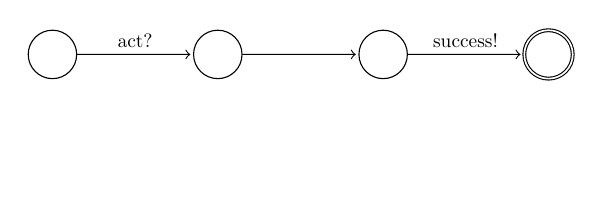
\begin{tikzpicture}[shorten >=1pt,node distance=3cm,on grid,auto,scale=0.7, font=\normalsize, every node/.style={transform shape}]
    
     \node[rectangle] (tmp) {};
     \node[state] (q_0) [above of=tmp, node distance=2cm]  {}; 
     \node[state] (q_1) [right of=q_0] {}; 
     \node[state] (q_2) [right of=q_1] {}; 
      \node[state,accepting](q_3) [right of=q_2] {};
 
   \path[->]
   
    (q_0) edge  node {act?} (q_1)
    (q_1) edge  node  {} (q_2)
    (q_2) edge  node  {success!} (q_3);
    
\end{tikzpicture}
\label{fig:bas}
}
&
\subfloat[AND gate]{
\centering
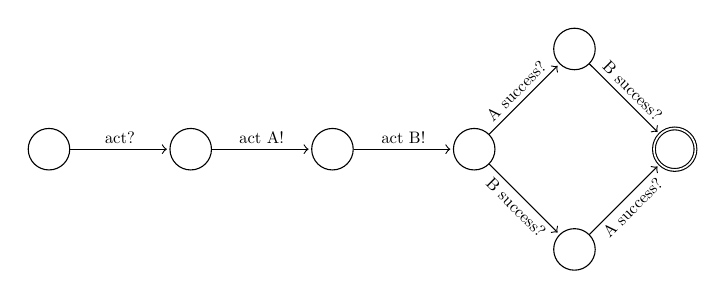
\begin{tikzpicture}[shorten >=1pt,node distance=3cm,on grid,auto,scale=0.6, font=\normalsize, every node/.style={transform shape}]
  
     \node[state] (q_0)  {}; 
     \node[state] (q_1) [right of=q_0] {}; 
     \node[state] (q_2) [right of=q_1] {}; 
     \node[state] (q_3) [right of=q_2] {};
      \node[state](q_4) [above right of=q_3] {};
  		\node[state](q_5)[below right of=q_3]{};
  		\node[state,accepting](q_6)[below right of=q_4]{};
  		
   \path[->]
   
    (q_0) edge  node {act?} (q_1)
    (q_1) edge  node  {act A!} (q_2)
    (q_2) edge  node  {act B!} (q_3)
    (q_3) edge  node [sloped, above] {A success?} (q_4)
    (q_3) edge  node [sloped, below]  {B success?} (q_5)
    (q_4) edge  node [sloped, above] {B success?} (q_6)
    (q_5) edge  node  [sloped, below] {A success?} (q_6);  
    
\end{tikzpicture}}
&
\subfloat[OR gate]{
\centering
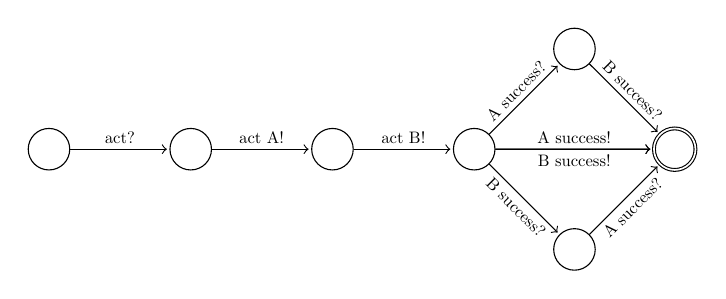
\begin{tikzpicture}[shorten >=1pt,node distance=3cm,on grid,auto,scale=0.6, font=\normalsize, every node/.style={transform shape}]
  
     \node[state] (q_0)  {}; 
     \node[state] (q_1) [right of=q_0] {}; 
     \node[state] (q_2) [right of=q_1] {}; 
     \node[state] (q_3) [right of=q_2] {};
      \node[state](q_4) [above right of=q_3] {};
  		\node[state](q_5)[below right of=q_3]{};
  		\node[state,accepting](q_6)[below right of=q_4]{};
  		
   \path[->]
   
    (q_0) edge  node {act?} (q_1)
    (q_1) edge  node  {act A!} (q_2)
    (q_2) edge  node  {act B!} (q_3)
    (q_3) edge  node [above] {A success!} (q_6)
    (q_3) edge  node [below] {B success!} (q_6)
    (q_3) edge  node[sloped, above] {A success?} (q_4)
    (q_3) edge  node [sloped, below]  {B success?} (q_5)
    (q_4) edge  node [sloped, above] {B success?} (q_6)
    (q_5) edge  node  [sloped, below] {A success?} (q_6);  
    
\end{tikzpicture}}
\\
\end{tabular}
}
\caption{Semantics of BAS and gates in terms of IMCs.}
\end{figure}


\section{Case Study and Interpretation of Results}
\tikzset{font=\scriptsize,
edge from parent fork down,
every node/.style=
    {rectangle,draw,fill=yellow!20,text width=1.0cm,
		text centered,font=\scriptsize,anchor=north}
}

\paragraph{Malicious Insider attack} The ACT for the malicious insider attack (MIA) from \cite{ACT} is depicted in Figure~\ref{fig:act}. The MIA ACT has BAS as well as detection and mitigation events. The countermeasure gates are represented by triangles. We conducted our case study by using the ADT toolbox \cite{ADT} to compare the results to \cite{ACT} and ATCalc \cite{ATCalc} to compute the attack probability over time. 

The result in Figure~\ref{result1} is obtained by varying all the probabilities of an attack in the leaf nodes (Pleaf) in the range of . Figure~\ref{result1} shows that with the countermeasures being in place, the probability of an attack at the root node (Pgoal) first decreases with only detection measures (perfect mitigation) and then increases with detection and mitigation measures in place (imperfect mitigation). Those results are equal to the results obtained in \cite{ACT}. To extend the case study, we consider now the probability of an attack over a time frame of  hours. Figure~\ref{result3} is obtained with different values for Pleaf, fixed at [0.05,0.1,0.25]. The results obtained in Figure~\ref{result3} shows that given an attacker ample time, it is sure that he will eventually be able to reach the goal. Further, it is nicely observable how much more time an attacker needs to reach his attack goal when the detection and mitigation is in place.

\begin{figure}[!t]
\begin{center}
\scalebox{0.95}{
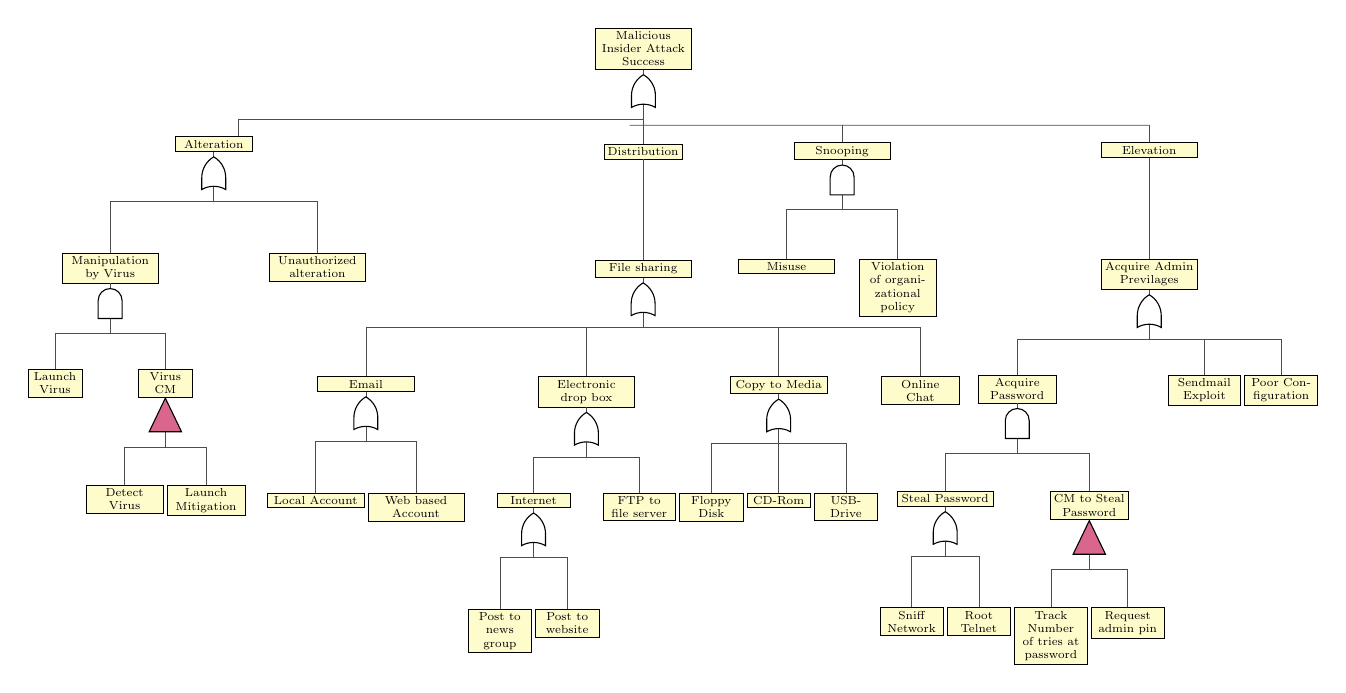
\begin{tikzpicture}[level 1/.style={sibling distance=.5cm},
and/.style={and gate US, draw,fill=white!60,rotate=90,
		anchor=east,xshift=-1mm},
    or/.style={or gate US,draw,fill=white!60,rotate=90,
		anchor=east,xshift=-1mm},
    be/.style={circle,draw,fill=white!60,anchor=north,
    font=\tiny, text width = 0.8cm, inner sep=0pt},
    tr/.style={buffer gate US,draw,fill=purple!60,rotate=90,
		anchor=east,minimum width=0.8cm},
label distance=3mm,
    every label/.style={blue},
event/.style={rectangle,draw,fill=yellow!20,text width=1.0cm,
		text centered,font=\scriptsize,anchor=north,inner sep=2pt},
edge from parent/.style={draw=black!70},
    edge from parent path={(\tikzparentnode.south) -- ++(0,-1.05cm)
			-| (\tikzchildnode.north)},
    level distance=70pt,
scale=0.6, font=\huge,every node/.style={transform shape}]]
\Tree [.\node[event,text width=1.9cm,xshift=2.795cm](G){Malicious Insider Attack Success}; 
[.\node[rectangle,xshift=-3cm](tmp2) {};  
	]         
[.\node[event,text width=1.5cm](A2){Distribution};
    [.\node[event,text width=1.9cm](A21){ File sharing};
    	[.\node[event,text width=1.9cm](A211){Email};
    		[.\node[event,text width=1.9cm](A2111){Local Account};]
    		[.\node[event,text width=1.9cm](A2112){Web based Account};]]
    	[.\node[event,text width=1.9cm](A212){Electronic drop box};
                                 [.\node[event,text width=1.4cm](A2122){Internet};
    									[.\node[event, text width=1.2cm](A21221){Post to news group};]
    									[.\node[event, text width=1.2cm](A2122){Post to website};]]
                                 [.\node[event,text width=1.4cm](A2121){FTP to file server};]]
               [.\node[event,text width=1.9cm](A214){Copy to Media};
                            [.\node[event, text width=1.2cm](A2141){Floppy Disk};]
                            [.\node[event, text width=1.2cm](A2142){CD-Rom};]
                            [.\node[event, text width=1.2cm](A2143){USB-Drive};]]
                [.\node[event,text width=1.5cm](A213){Online Chat};]]]		 
]

\begin{scope}[xshift=13.5cm,yshift=-2.43cm]
\node[rectangle,yshift=.365cm] (tmp3) {};
\Tree 
[.\node[event,text width=1.9cm](A4) {Elevation};  
			[.\node[event,text width=1.9cm](A41){Acquire Admin Previlages};
				   [.\node[event,text width=1.5cm](R){Acquire Password};
		             		  	[.\node[event,text width=1.9cm](A412){Steal Password};
									[.\node[event,text width=1.2cm](A4121){Sniff Network};]
									[.\node[event,text width=1.2cm](A4122){Root Telnet};]]
		                        [.\node[event,text width=1.5cm](S){CM to Steal Password};
									[.\node[event,text width=1.4cm](D412){Track Number of tries at password};]
									[.\node[event,text width=1.4cm](M412){Request admin pin};]]]
		[.\node[event,text width=1.4cm](A413){Sendmail Exploit};]
		[.\node[event,text width=1.4cm](A41){Poor Configuration};]]]	
\end{scope}

\begin{scope}[xshift=-6.3cm,yshift=-2.3cm]
\Tree 
[.\node[event,text width=1.5cm](A1) {Alteration};  
	[.\node[event,text width=1.9cm](P){Manipulation by Virus};
	                   [.\node[event](A12){Launch Virus};]
            		   [.\node[event](Q){Virus CM};
             		  	   [.\node[event,text width=1.5cm](D12){Detect Virus};]
             		  	   [.\node[event,text width=1.5cm](M12){Launch Mitigation};]]]
     [.\node[event, text width=1.9cm](A11){Unauthorized alteration};]]      
\end{scope}

\begin{scope}[xshift=7cm,yshift=-2.43cm]
\node[rectangle,yshift=.365cm] (tmp) {};
\Tree 
[.\node[event,text width=1.9cm](A3){Snooping};
		[.\node[event,text width=1.9cm](A31){Misuse};] 
		[.\node[event,text width=1.5cm](A32){Violation of organizational policy};]]
\end{scope}

\node[left of=tmp, node distance=4.5cm] (tmp4) {};

\path[-] (A3.north) edge[line width=0.2pt,color=black!70] (tmp.center);
\path[-] (A4.north) edge[line width=0.2pt,color=black!70] (tmp3.center);
\path[-] (tmp4.center) edge[line width=0.2pt,color=black!70] (tmp3.center);
		
\node [or]	at (G.south)	[]	{};
\node [or]	 at (A1.south)	[]	{};
\node [and]	at (P.south)	[]	{};
\node [tr]  at (Q.south)	[]	{};
\node [and]  at (A3.south)	[]	{};
\node [or]	at (A21.south)	[]	{};
\node [or]	at (A211.south)	[]	{};
\node [or]	at (A212.south)	[]	{};
\node [or]	at (A2122.south)	[]	{};
\node [or]	at (A214.south)	[]	{};
\node [or]	at (A41.south)	[]	{};
\node [and]	at (R.south)	[]	{};
\node [or]	at (A412.south)	[]	{};
\node [tr]	at (S.south)	[]	{};

\end{tikzpicture}}
\end{center}
\caption{ACT of the malicious insider attack.}
\label{fig:act}
\end{figure}

\begin{figure}[ht!]
\scalebox{0.85}{
    \subfloat[Pgoal versus Pleaf]{
\begin{tikzpicture}[scale=1,font=\tiny,every node/.style={transform shape}]
	\begin{axis}[ymin=0,xmin=0,xmax=1,ymax=1,grid = both,
	xlabel=Pleaf,
	ylabel=Pgoal,
	ylabel shift = 2pt, legend pos=south east,
	cycle list name=mycolorlist]

	\addplot table {simulation_case_ADT_1.dat};
	\addlegendentry{No CM}	
	
	\addplot table {simulation_case_ADT_2.dat};
	\addlegendentry{With CM (Detect and Mitig)}	
	
	\addplot table {simulation_case_ADT_3.dat};
	\addlegendentry{Only Detect}	
		\end{axis}
\end{tikzpicture}
        \label{result1}
   }
    \hspace{1cm}
   \subfloat[Pgoal versus Time]{
\begin{tikzpicture}[scale=1,font=\tiny,every node/.style={transform shape}]
	\begin{axis}[ymin=0,xmin=0,xmax=10,ymax=1,grid = both,
	xlabel=Time,
	ylabel=Pgoal,
	ylabel shift = 1cm, legend pos=south east,
	cycle list name=mycolorlist]

	\addplot table {simulation_case_AT_Calc_1.dat};
	\addlegendentry{{Without CM (P=0.05)}}	
	
	\addplot table {simulation_case_AT_Calc_2.dat};
	\addlegendentry{{Without CM (P=0.01)}}	
	
	\addplot table {simulation_case_AT_Calc_3.dat};
	\addlegendentry{{Without CM (P=0.25)}}	
	
	\addplot table {simulation_case_AT_Calc_4.dat};
	\addlegendentry{{CM-Detect (P=0.05)}}	
	
	\addplot table {simulation_case_AT_Calc_5.dat};
	\addlegendentry{{CM-Detect (P=0.1)}}	
	
	\addplot table {simulation_case_AT_Calc_6.dat};
	\addlegendentry{{CM-Detect (P=0.25)}}	
	
	\addplot table {simulation_case_AT_Calc_7.dat};
	\addlegendentry{{CM-Detect+Mitig (P=0.05)}}	
	
	\addplot table {simulation_case_AT_Calc_8.dat};
	\addlegendentry{{CM-Detect+Mitig (P=0.1)}}	
	
	\addplot table {simulation_case_AT_Calc_9.dat};
	\addlegendentry{{CM-Detect+Mitig (P=0.25)}}	
	
	\end{axis}
\end{tikzpicture}
        \label{result3}
    }}
    \caption{ versus (a)   (b) Time(sec)}
\end{figure}

\section{Conclusion}
We presented the inclusion of time in Attack Countermeasure trees and provided a case study to show the applicability of this approach. This enables us to answer questions like: What is the probability for an attacker to succeed given  time units by integrating new countermeasures? In future work we consider shared attack scenarios as well as extend the dynamic ACTs with:
\begin{inparaenum}[(\arabic{enumi})]
\item Sequential AND and Sequential OR gates which can model the casual dependencies of attack steps, i.e. an attack can only take place if attack steps are executed in a certain order;
\item  Probabilistic gates which activates the BAS and countermeasure events with discrete probabilities, i.e. attacks as well as countermeasures are only executed with a certain probability.\end{inparaenum}

\paragraph{Acknowledgement.} This work has been supported by the EU FP7 project TREsPASS (318003) and by the STW-ProRail partnership program ExploRail under the project ArRangeer (12238). 

\bibliographystyle{eptcs}
\bibliography{mybiblo}


\end{document}
